\label{sec:method}

\begin{wrapfigure}{r}{.31\textwidth}
\vspace{-8mm}
\begin{center}
    \centering
    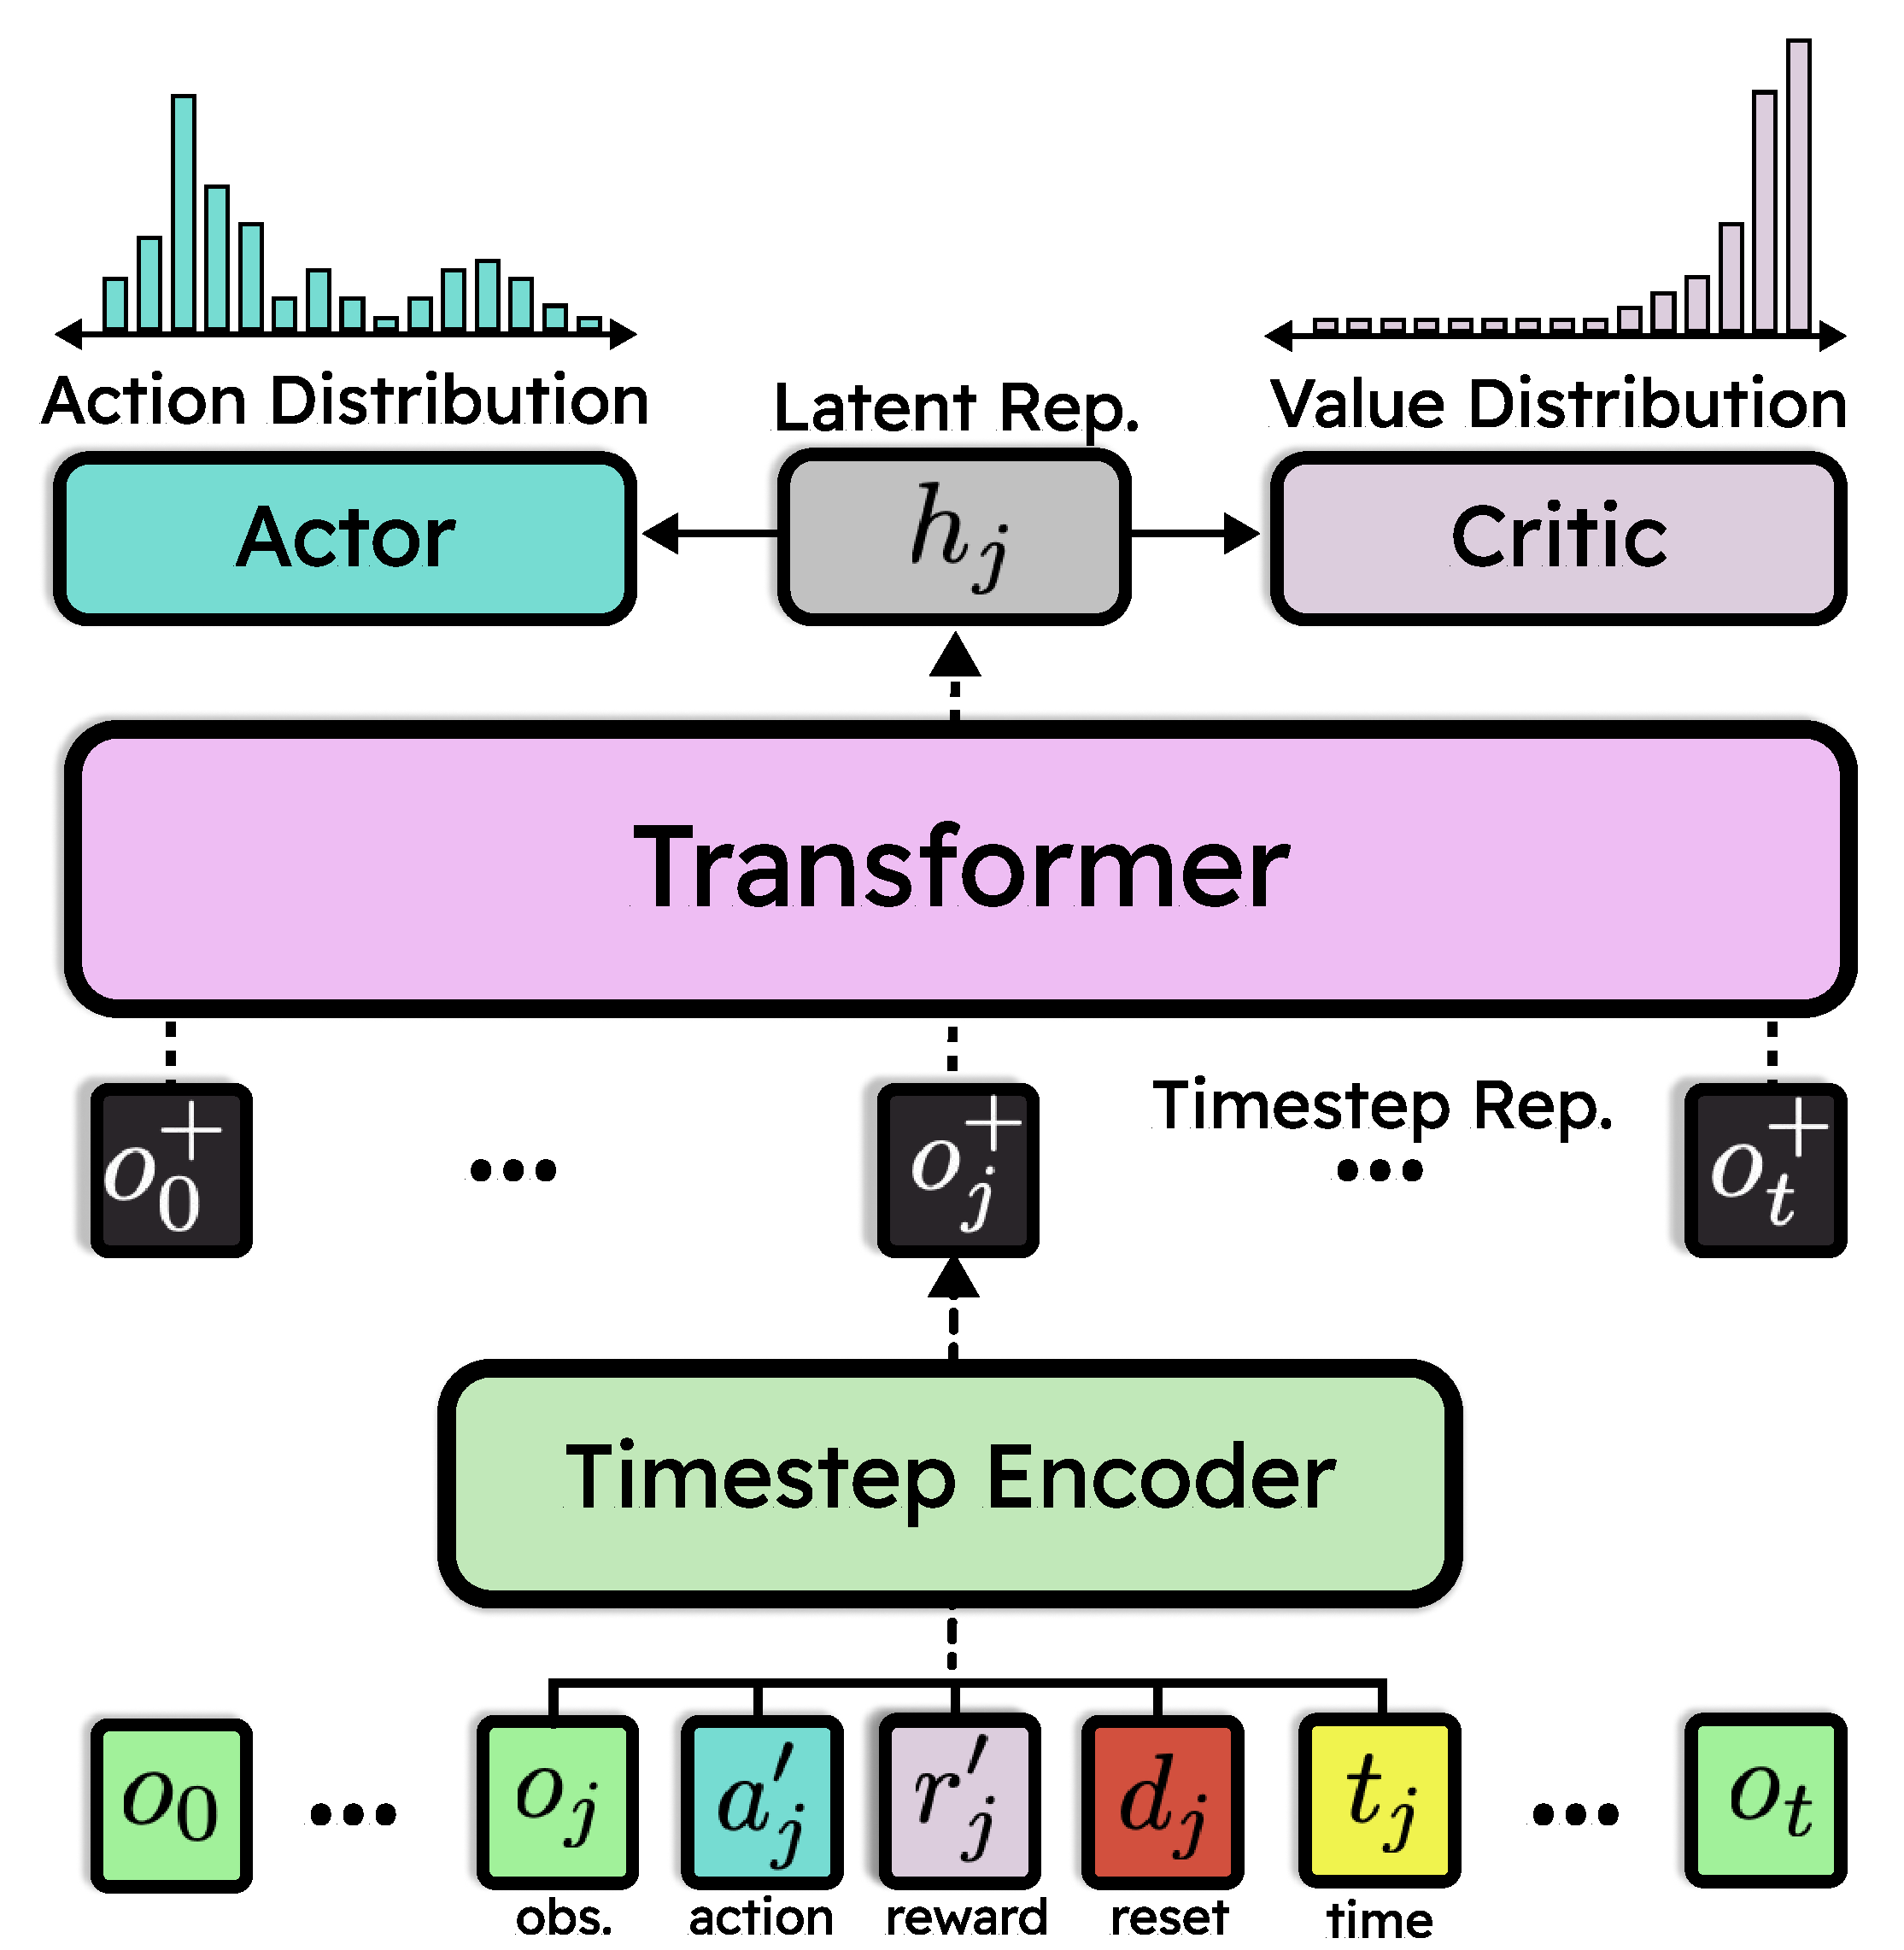
\includegraphics[width=.3\textwidth]{figures/final/arch_fig_v4.pdf}
    \vspace{-3mm}
    \caption{\textbf{Transformer-based Actor-Critic Architecture.}}
    \label{fig:arch}
\end{center}
\vspace{-6mm}
\end{wrapfigure}
We study multi-task adaptation without task labels by building on the flexible memory-based framework in which sequence models optimize standard RL objectives across trajectory inputs (Section \ref{sec:background}). Agents observe trajectory slices from a replay buffer with a context length of up to $l$ timesteps ($\tau_{t-l:t}$). The information revealed between timesteps ($o_i, a_{i-1}, r_{i -1}, d_{i -1})$ is merged into a single embedding $o^+_i$. The sequence $(o^+_{t-l}, \dots, o^+_t)$ is then passed through a sequence-to-sequence model to produce $(h_{t-l}, \dots, h_t)$ which serves as a shared representation for output heads representing the critic(s) $Q$ and stochastic policy $\pi$ (Figure \ref{fig:arch}). We focus on the combination of Transformers and off-policy RL updates, which will let us evaluate large-scale policies trained over millions of timesteps. Let $y_t = r_{t} + \gamma \bar{Q}(h_{t+1}, a' \sim \bar{\pi}(h_{t+1}))$ be the one-step temporal difference target, where $\bar{Q}$ and $\bar{\pi}$ refer to frozen target networks \cite{lillicrap2015continuous}. We can  minimize standard off-policy actor-critic loss terms \cite{lillicrap2015continuous, christodoulou2019soft} in parallel over the context length:

\begin{minipage}{0.45\textwidth}
  \begin{align}
    \label{eq:critic_dep}
    \mathcal{L}_{\text{Critic}}(t) &= \left(Q(h_t, a_t) - y_t\right)^2 
    \end{align}
\end{minipage}
\begin{minipage}{0.45\textwidth}
    \begin{align}
     \label{eq:actor_dep}
     \mathcal{L}_{\text{Actor}}(t) &= -Q\big(h_t, a \sim \pi(h_t)\big)
    \end{align}
\end{minipage}

Following details in AMAGO \cite{grigsby2024amago}, we compute Equations \eqref{eq:critic_dep} and \eqref{eq:actor_dep} with an ensemble of critics \cite{chen2021randomized} and over several different values of the discount factor $\gamma$ in parallel \cite{fedus2019hyperbolic}. By preventing the parameters of $Q$ from minimizing $\mathcal{L}_{\text{Actor}}$, we can update the full architecture with one step of the joint loss: $\sum_{i = t-l}^{t-1}\mathcal{L}_{\text{Actor}}(i) + \lambda \mathcal{L}_{\text{Critic}}(i)$, where $\lambda$ is a hyperparameter that balances the objectives for the shared sequence model \cite{ni2023transformers, grigsby2024amago}.


Multi-task optimization challenges are not unique to RL \cite{shaham2023causes, royer2024scalarization}, but RL typically adds a bottleneck that we can remove: both Equations \eqref{eq:critic_dep} and \eqref{eq:actor_dep} directly depend on the scale of returns $Q$ in each of our $N$ tasks. When computed as a simple expectation over tasks, the gradients of $\mathcal{L}_{\text{Critic}}$ and $\mathcal{L}_{\text{Actor}}$ can favor small \textit{relative} improvements in tasks with high \textit{absolute} returns (Figure \ref{fig:relative_losses} left). We can almost never assume tasks have similar return scales. For example, even when we design reward functions to have similar initial and optimal returns, differences in task difficulty lead to uneven learning progress and imbalanced $Q$-values. This issue was proposed and demonstrated by methods such as Multi-Task PopArt \cite{hessel2019multi}. PopArt's solution is to compute MTRL loss terms on a relative basis by creating a new critic output for each of the $N$ tasks. Each critic adaptively normalizes $y$ for its task and automatically rescales its output to help compensate for shifting targets. Simpler versions of this approach (e.g., without network rescaling) are universal in MTRL. However, we cannot use this technique without ground-truth knowledge of task labels. Although we cannot adaptively balance each task's loss, we can reformulate Eqs. \eqref{eq:critic_dep} and \eqref{eq:actor_dep} to be less sensitive to the scale of $Q$. 



\paragraph{Scale-Resistant Critics.} Distributional RL \cite{bellemare2023distributional} is motivated by representation learning and risk-aware policies, but methods like C51 \cite{bellemare2017distributional} have a useful side-effect of turning \eqref{eq:critic_dep} into a classification problem that scales with the number of output bins instead of $Q$. For this reason, C51-style critic updates have become a key implementation detail in large-scale (offline) MTRL agents \cite{kumar2022offline, springenberg2024offline}. We can keep the classification side-effect without modeling return distributions by converting a scalar $Q$ to discrete label(s) $\in \{0, \dots, B\}$. Two-hot labels create a one-to-one mapping between every scalar in a fixed range and a discrete distribution where all non-zero probability is placed in two adjacent bins \cite{schrittwieser2020mastering, hessel2021muesli}. If $Q_B$ denotes a modified critic network that outputs probabilities over $B$ bins, the TD-error can be minimized by multi-label classification:

\vspace{-5mm}
\begin{align}
    \label{eq:critic_ind}
    \mathcal{L}_{\text{Critic-Ind}}(t) = -\text{twohot}_B(y_t)^\mathsf{T} \log Q_B(h_t, a_t)
\end{align}
\vspace{-5mm}

\begin{wrapfigure}{r}{.61\textwidth}
\vspace{-8mm}
\begin{center}
    \centering
    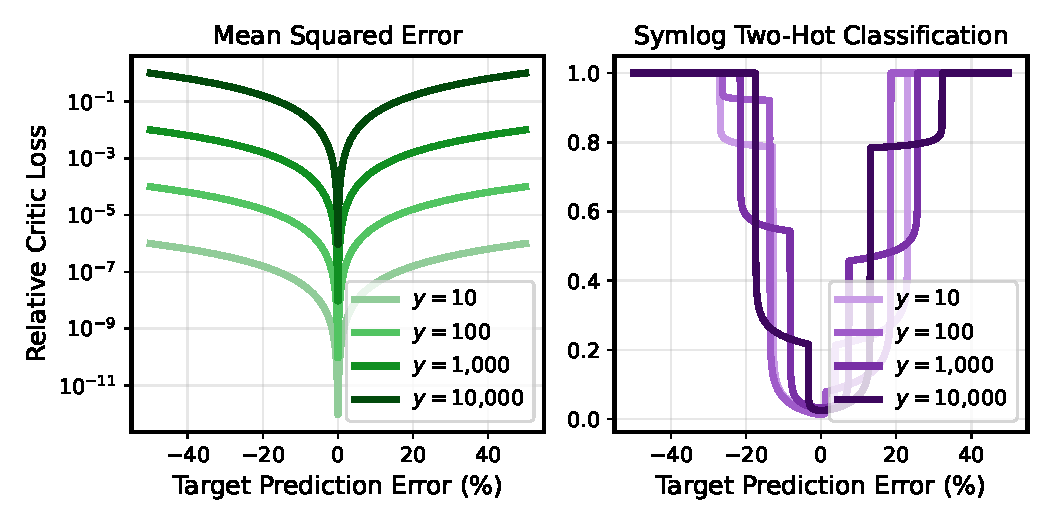
\includegraphics[width=.6\textwidth]{figures/final/condensed_twohot_prediction_error.pdf}
    \vspace{-4mm}
    \caption{\textbf{Scale-Resistant Value Regression.} We plot the value of the standard critic loss (Eq. \ref{eq:critic_dep}) as a function of the \textit{relative} prediction error of the TD target ($y$) across four orders of magnitude (left). Y-axes are self-normalized according to the largest displayed value. Two-Hot classification (Eq. \ref{eq:actor_ind}) maps the same relative error to similar loss values across the different absolute return scales of each task (right).}
    \label{fig:relative_losses}
\end{center}
\vspace{-4mm}
\end{wrapfigure}

We can reduce tuning of label spacing and limits with an invertible transform that maps a wide range of returns to a smaller number of labels \cite{kapturowski2018recurrent}; we use \texttt{symlog} as demonstrated by DreamerV3 \cite{hafner2023mastering} and TD-MPC2 \cite{hansen2023td}. We also experimented with using a global (task-agnostic) $Q$-normalization for this purpose but found that a fixed mapping is important because stabilizing learning against shifting labels required extensive hyperparameter tuning. Figure \ref{fig:relative_losses} visualizes why we would expect classification to be an improvement in a multi-task setting: $\mathcal{L}_{\text{Critic-Ind}}$ maps the same relative error in value prediction to a similar loss value over a wide range return scales. In contrast, $\mathcal{L}_{\text{Critic}}$ can bias optimization towards tasks that happen to have large regression targets. This effect can be dependent on proper tuning of the bin count $B$, upper/lower return bounds, and use of the \texttt{symlog} transform (Appendix \ref{app:implementation}).


A concurrent work \cite{farebrother2024stop} evaluates the two-hot critic loss' ability to unlock scaling laws in RL when used as a direct replacement for $\mathcal{L}_{\text{Critic}}$ \eqref{eq:critic_dep} (or its algorithm-specific equivalent). They find the classification loss improves performance in a range of domains and attribute this to advantages in representation learning and robustness to noisy value targets ($y$). Our experiments focus on the PopArt hypothesis that scale-invariance improves optimization in an online multi-task setting. We will be exploring the impact of classification losses in an actor-critic agent with adaptive memory, where we also need to consider the scale of the policy's objective \eqref{eq:actor_dep}.


\paragraph{Scale-Resistant Actors.} Many policy updates resemble a weighted regression objective where the importance of each action label is scaled by a function $f(\tau, a)$ that increases with its value or advantage, such as $f(\tau, a) \propto \exp(A(\tau, a))$\footnote{Where $A(\tau, a) = Q(\tau, a) - Q(\tau, a' \sim \pi(\tau))$ is the improvement of $a$ over the value of the current policy as estimated by actor and critic networks that take trajectory sequences as input.}. Methods differ in where the candidate actions $a$ are sampled from, how values are estimated, and how $f(\tau, a)$ clips or rescales the update \cite{hessel2021muesli, schulman2017proximal, abdolmaleki2018maximum, peng2019advantage, wang2018exponentially}. In the off-policy setting where actions are sampled from a dataset of previous experience, slight differences in advantage estimates and weight functions $f$ create a dense family of similar advantage-weighted regression (AWR) methods \cite{peng2019advantage, wang2018exponentially, chen2020bail, siegel2020keep, grigsby2021closer}. AWR is intuitive and simple to implement but directly depends on the scale of returns unless we intentionally avoid this with a binary filter $f(\tau, a) = \mathbbm{1}\{A(\tau, a) > 0\}$ \cite{wang2020critic, nair2018overcoming}. We follow details from CRR-Binary-Mean \cite{wang2020critic} for a candidate actor loss that is independent of $Q$:

\vspace{-4mm}
\begin{align}
    \label{eq:actor_ind}
    \mathcal{L}_{\text{Actor-Ind}}(t) = -\mathbbm{1}\{Q(h_t, a_t) - \mathop{\mathbb{E}}_{a' \sim \pi(h_t)}[Q(h_t, a')] > 0\}\log\pi(a_t \mid h_t)
\end{align}
\vspace{-4mm}

Intuitively, CRR performs imitation learning (IL) on action labels that we estimate will improve the current policy. Advantage estimates within $\mathcal{L}_{\text{Actor-Ind}}$ rely entirely on one-step dynamic programming \eqref{eq:critic_dep} so that they never become outdated \cite{wang2020critic, nair2020awac}. Because they do not allow the policy to extrapolate to out-of-distribution actions, weighted IL updates like CRR are best suited to \textit{offline} RL \cite{levine2020offline}. In offline RL, the ability to stabilize optimization on static datasets is well worth losing the optimistic exploration of $\mathcal{L}_{\text{Actor}}$ \eqref{eq:actor_dep}. Choosing to use $\mathcal{L}_{\text{Actor-Ind}}$ online implies that the ability to address issues in multi-task optimization is a similarly worthwhile trade-off. There are other RL engineering factors to consider in the specific case of training long-context Transformers. For example, sampling batches of trajectory sequences can create replay ratios high enough to effectively be offline RL \cite{fedus2020revisiting}. However, the simplest justification for training Transformers on $\mathcal{L}_{\text{Actor-Ind}}$ may come from its similarities to widely used methods for supervised learning in RL.

\paragraph{Transformers and RL via Supervised Learning.} Decision Transformer (DT) is a popular approach to training sequence policies that reformulates RL as IL conditioned on a target return \cite{chen2021decision, janner2021reinforcement, lee2022multi}. DT's advantage is that it reduces to IL on expert datasets, making it a safe improvement over a technique that is already effective for many problems. In a field where engineering is critical, and results can be hard to reproduce, there is valuable simplicity in inheriting technical details from supervised sequence modeling. This simplicity has likely contributed to the method's success despite several disadvantages. For example, DT policies are conditioned on the optimal return in order to imitate the best continuation of the current trajectory, but $\mathcal{L}_{\text{Actor-Ind}}$ does this without needing to define the optimal return in advance. DT determines the value of an action based on the fixed return of its trajectory, while $\mathcal{L}_{\text{Actor-Ind}}$ continuously updates its estimate with the value of the current network. By extension, DT cannot handle stochastic reward functions \cite{paster2022you}. Like DT, $\mathcal{L}_{\text{Actor-Ind}}$ becomes IL on expert datasets, and Eqs.~\eqref{eq:critic_ind} and \eqref{eq:actor_ind} resemble supervised learning with two classification heads.